% --------------------------------------------------------------------
% Beamer Template 
% --------------------------------------------------------------------
% Necessary infos for documentstyle
\documentclass[compress]{beamer}

\usetheme{Stud}
\usepackage{times}
\usepackage[utf8]{inputenc}
\usepackage[T1]{fontenc} % nicht benoetigt, in folien wird eh nicht getrennt
\usepackage{ngerman}
\usepackage{graphicx}
%\usepackage{color}% color wird bereits von beamer geladen
\usepackage{verbatim}
\usepackage{psfrag}
\usepackage{math}
\usepackage{calc}
\usepackage{tabularx}
\usepackage{enumerate}


% --------------------------- Helpers ----------------------------
% to use these texts in two languages
% changes the parameter within {#}
% 1 = German
% 2 = English
\def\twolang#1#2{#1} 
\let\2=\twolang

% --------------------------------------------------------------------


\bibliographystyle{alphadin}
\graphicspath{{images/}}


% --------------------------------------------------------------------
\title{Antrittsvortrag zur Bachelorarbeit}
\subtitle{}
\author[T. Budweg]{Tim Budweg}
\institute{
  \texttt{tbudweg@uni-koblenz.de} \\
  \vspace{0.2cm}
  \2{AG Rechnernetze\\
  Universität Koblenz-Landau}{Institute for Computer Science\\
  University of Koblenz and Landau}
}
\date{3. Juni 2015}
% --------------------------------------------------------------------



% document
\begin{document}

\frame{\titlepage}

%\logo{...} erst hier, damit es nicht mit auf die Titelseite kommt!
\logo{\pgfuseimage{logo}}

\part{Overview}
\section{\2{Überblick}{Overview}}
\frame{
  \frametitle{\2{Überblick}{Overview}}
  \tableofcontents[part=2,hideallsubsections]
}

% ====================================================================
% ====================================================================

% here comes the real content which is part of scontent.tex
\part{Content}

% ---------------------------------------------------------------------------
% - For showing graphics and text on one slide use:
%   \begin{columns}[T]
%	\begin{column}[T]{.5\linewidth}
%	    \includegraphics[width=\linewidth]{<filename>}
%	\end{column}
%	\begin{column}[T]{.5\linewidth}
%	    <content>
%	\end{column}
%   \end{columns}
% ---------------------------------------------------------------------------

\section{Einleitung}

\subsection{l}
\begin{frame}
Thema:\\
	Reaktive Konstruktion eines planaren t-Spanners mit konstantem Knotenausgangsgrad
\end{frame}

\subsection{Motivation}
\begin{frame}
\begin{itemize} % reaktive Algorithmen ohne constant node degree->nicht so energieeffizient wie mit
	\item reaktive Algorithmen, welche einen t-Spanner erzeugen (PDT)
	%ohne t-Spanner->mögliche lange Umwege
	\item reaktive Algorithmen mit konstantem Ausgangsgrad () Beispiel
\end{itemize}
\end{frame}
\subsection{}
\begin{frame}
	\begin{itemize}
		\item $LDel^{(2)}(U) $
		\item Modified Yao Step 
	\end{itemize}
\end{frame}

\subsection{$LDel^{(2)}(U) $}
\begin{frame}
\begin{itemize}
    \begin{columns}[T]
	\begin{column}[T]{.5\linewidth}
    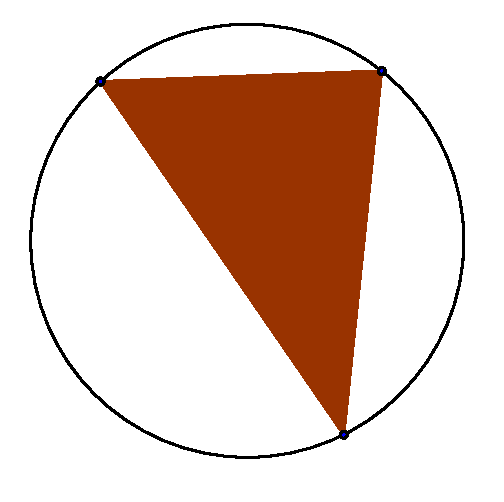
\includegraphics[width=\linewidth]{Dreieck.eps}
	\end{column}
	\begin{column}[T]{.5\linewidth}
	    \item alle Dreiecke, welche keine 2-Hop-Nachbarn in ihrem Umkreis beinhalten
	    
	\end{column}
   \end{columns}
\end{itemize}
\end{frame}

\subsection{Modified Yao Step}
\begin{frame}
  Input: $LDel^{(2)}(U) $
	\begin{itemize}
    \begin{columns}[T]
	\begin{column}[T]{.5\linewidth}
    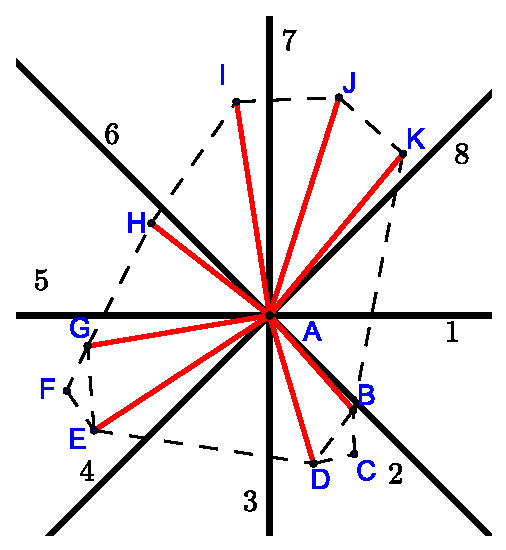
\includegraphics[width=\linewidth]{finished_A.eps}
	\end{column}
	\begin{column}[T]{.5\linewidth}
	    \item Bilde Kegel
	    \item Wähle Kanten aus
	\end{column}
   \end{columns}
	\end{itemize}
\end{frame}

\section{Ziele}
\subsection{}
\begin{frame}
Folgende Eigenschaften müssen erfüllt sein:
\begin{itemize}
  \item Ergebnisgraph ist ein euklidischer t-Spanner
  \item Ergebnisgraph ist planar
  \item Der Knotenausgangsgrad ist konstant beschränkt
  \item reaktive Konstruktion des Graphen
  \item Der Algorithmus muss streng lokal arbeiten
\end{itemize}
\end{frame}



\section{Bisherige Ergebnisse}
\subsection{}
\begin{frame}
	Beweis, dass PDT alle Eigenschaften erfüllt, die $LDel^{(2)}(U) $ erfüllt 
\end{frame}

\subsection{reactive Modified Yao Step}
\begin{frame}
Input: planarer, t-spanner (PDT)
Output: zusätzlich konstanter Ausgangsgrad
	\begin{enumerate}
		\item bilde Kegel
		\item finde kürzeste Kante \ldots
		\item finde eine zusätzliche Kante für jeden leeren Kegel
		\item Prüfe, ob beide Endpunkte einer Kante diese akzeptieren
	\end{enumerate}
\end{frame}

\subsection{finde kürzeste Kante}
\begin{frame}
\begin{itemize}
	\item stelle Timer in Abhängigkeit zur Distanz eines Knotens
	\item Beim Hören einer Nachricht:
	\begin{itemize}
		\item falls in selbem Kegel -> breche Timer ab
		\item sonst -> nop
	\end{itemize}
\end{itemize}
\end{frame}

\end{document}
